\chapter{反应进度表}\label{ch:g10:reaction-progress-table}

% ledger: use:NaN3-airbag
在一次汽车碰撞中，方向盘中的气囊弹出，
并在不到一秒的时间内充满气体，早于驾驶员头部前冲。
气体由一次化学反应生成：一小块固体，
经典设计中为叠氮化钠，分解为钠和氮气。
工程师必须放入足够的固体以充满气囊，
但不能放得太多以致气囊爆裂，且不能残留任何会伤害
乘员的反应物。多少固体能产生多少气体？配平的方程式给出
各物质的比例；本章将其转化为一种记账工具，
用以跟踪反应从开始到结束过程中的每一种反应物
和生成物。

\begin{recall}
配平的方程式使每种元素的原子数以及电荷
在等式两边保持相同；其化学计量数给出各物种反应的
比例（见\cref{ch:g8:balanced-equations}）。某物种的物质的量
对于质量，$n = m/M$；对于气体，$n = V/V_m$
（其中 $V_m = \qty{24.1}{L/mol}$，取值条件为 \qty{20}{\celsius} 和常压）
（见\cref{ch:g10:the-mole}）；对于溶质，$n = c \times V$
（见\cref{ch:g10:concentration-and-dilution}）。
\end{recall}

\begin{omfigure}
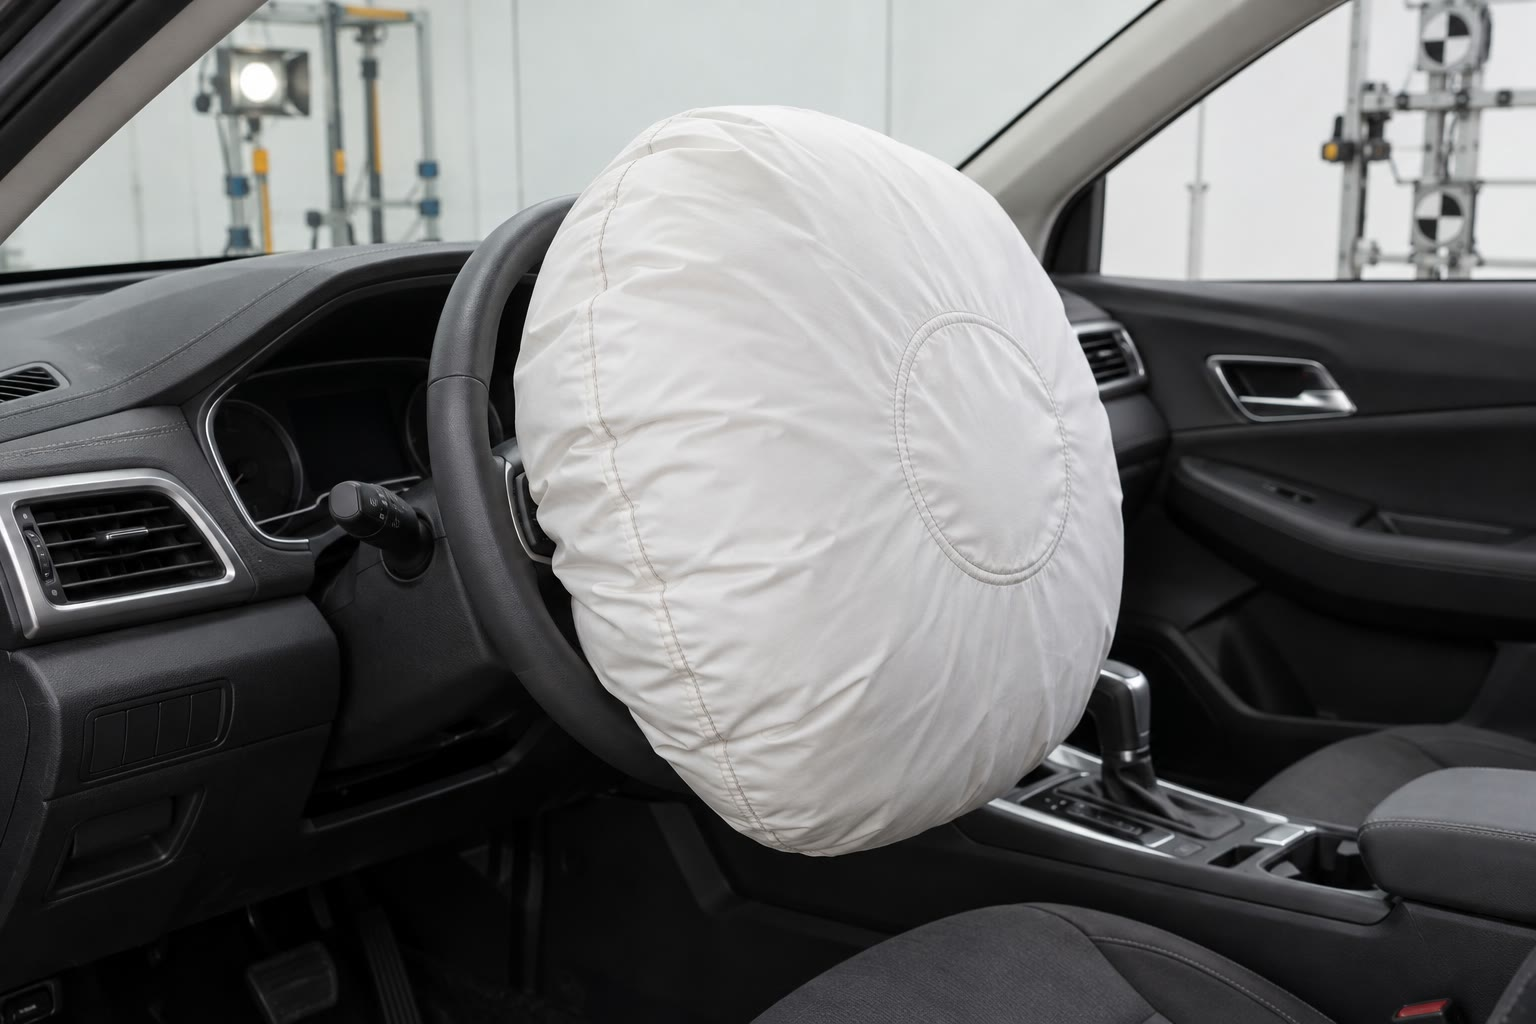
\includegraphics[width=0.5\linewidth]{images/book1/ai/g10-airbag.jpg}

{\small 气囊在不到一秒内充满，其中的氮气
由反应生成。}
\end{omfigure}

\section{描述化学体系}

\begin{definition}[化学体系，初始状态与最终状态]\label{def:g10:reaction-progress-table:system}
称\emph{化学体系}\index{化学体系}为
给定空间（如烧瓶、气囊、电池）中存在的全部化学物种的集合，
每种物种都有其物质的量和物理状态。反应开始前的体系
称为\emph{初始状态}\index{初始状态}；
反应停止后的体系称为\emph{最终
状态}\index{最终状态}。
\end{definition}


\begin{example}[密闭容器中的甲烷燃烧]\label{ex:g10:reaction-progress-table:methane}
密闭容器中含有 \qty{2.0}{mol} 甲烷和 \qty{3.0}{mol}
氧气；火花引发燃烧反应
\ce{CH4 + 2O2 -> CO2 + 2H2O}。在初始状态下，体系中含有
\qty{2.0}{mol} \ce{CH4(g)}、\qty{3.0}{mol} \ce{O2(g)} 且没有
生成物。最终状态是什么？本章其余部分将给出答案。
\end{example}

\section{反应进度与进度表}

\begin{definition}[反应进度，进度表]\label{def:g10:reaction-progress-table:extent}
称\emph{反应进度}\index{反应进度} $x$（单位为摩尔）
为反应按配平方程式所写的进行次数：
反应进度为 $x$ 时，某化学计量数为 $\nu$ 的物种
已被消耗（反应物）或生成（生成物）了 $\nu x$ 的物质的量。
\emph{进度表}\index{进度表}在方程式下方，给出
初始状态下，
反应进度为 $x$ 时以及最终状态下每种物种的物质的量。
\end{definition}

\begin{method}[填写进度表]\label{met:g10:reaction-progress-table:fill}
\begin{enumerate}
  \item 在第一行写出配平的方程式。
  \item 初始状态（$x = 0$）：在其下方写出每种物种
        的初始物质的量。
  \item 中间状态（反应进度为 $x$）：化学计量数
        为 $\nu$ 的反应物变为 $n_0 - \nu x$，生成物变为 $n_0 + \nu x$。
  \item 最终状态：求出 $x_{\max}$（见下一节），并将其代入
        中间状态一行的表达式。
\end{enumerate}
\end{method}

\begin{omfigure}
\renewcommand{\arraystretch}{1.25}
\begin{tabular}{l|c|cccc}
\hline
方程式 & & \ce{CH4} & $+$ \ce{2O2} & $\longrightarrow$ \ce{CO2} & $+$ \ce{2H2O} \\
\hline
状态 & 反应进度（\si{mol}） & \multicolumn{4}{c}{物质的量（\si{mol}）} \\
\hline
初始 & $0$ & $2.0$ & $3.0$ & $0$ & $0$ \\
中间 & $x$ & $2.0 - x$ & $3.0 - 2x$ & $x$ & $2x$ \\
最终 & $x_{\max} = 1.5$ & $0.5$ & $0$ & $1.5$ & $3.0$ \\
\hline
\end{tabular}\par\medskip

{\small 例中甲烷燃烧的进度表。
每列对应一种物种；\ce{O2} 与
\ce{H2O} 的系数 2 均变为 $2x$。}
\end{omfigure}

\section{限量反应物与最终状态}

\begin{definition}[限量反应物，最大反应进度，完全反应]\label{def:g10:reaction-progress-table:limiting}
若一个反应仅当其某一反应物耗尽时才停止，则称之为
\emph{完全反应}\index{完全反应}。
该反应物称为\emph{限量反应物}\index{限量反应物}；
其他反应物则过量。限量反应物恰好耗尽时的反应进度
称为\emph{最大反应进度}\index{最大反应进度} $x_{\max}$；
完全反应的最终状态即为 $x = x_{\max}$ 时的状态。
\end{definition}

\begin{method}[求限量反应物]\label{met:g10:reaction-progress-table:limiting}
\begin{enumerate}
  \item 对每种反应物，解 $n_0 - \nu x = 0$：该反应物将
        在 $x = n_0 / \nu$ 时耗尽。
  \item 这些值中最小者即为 $x_{\max}$；给出该值的反应物
        即为限量反应物。
  \item 将 $x_{\max}$ 代入中间状态一行，求得最终状态；
        检查各物质的量是否为负值。
\end{enumerate}
\end{method}

\begin{example}[回到甲烷]\label{ex:g10:reaction-progress-table:methane-final}
甲烷将在 $x = 2.0/1 = \qty{2.0}{mol}$ 时耗尽，氧气则在
$x = 3.0/2 = \qty{1.5}{mol}$ 时耗尽。较小者为 \qty{1.5}{mol}：氧气是
限量反应物，$x_{\max} = \qty{1.5}{mol}$。最终状态
中剩余甲烷 \qty{0.5}{mol}，没有氧气，
生成 \qty{1.5}{mol} 二氧化碳和 \qty{3.0}{mol} 水。
\end{example}

\begin{omfigure}
\begin{tikzpicture}
\begin{axis}[width=0.78\linewidth, height=6.2cm, xmin=0, xmax=2.05,
    ymin=0, ymax=4.2, xlabel={反应进度 $x$ (\si{mol})},
    ylabel={物质的量 (\si{mol})}, axis lines*=left, ymajorgrids,
    grid style={gray!20}, tick label style={font=\small},
    label style={font=\small}, xtick={0,0.5,1,1.5,2},
    legend style={font=\small, at={(1.02,0.5)}, anchor=west, draw=none},
    legend cell align=left]
  \addplot[very thick, omDef, domain=0:2] {2-x};
  \addplot[very thick, omThm, domain=0:1.5] {3-2*x};
  \addplot[very thick, omMeth, domain=0:2] {x};
  \addplot[very thick, omProp, domain=0:2] {2*x};
  \legend{\ce{CH4}, \ce{O2}, \ce{CO2}, \ce{H2O}}
  \addplot[dashed, black!60] coordinates {(1.5,0) (1.5,4.2)};
  \node[font=\small, anchor=south west] at (axis cs:1.5,3.55) {$x_{\max}$};
  \fill[black!8, opacity=0.6] (axis cs:1.5,0) rectangle (axis cs:2.05,4.2);
\end{axis}
\end{tikzpicture}

{\small 甲烷示例中物质的量随反应进度的变化。氧气
（红色）最先降至零，此时 $x = \qty{1.5}{mol}$，反应
在此停止，阴影部分永远不会达到。}
\end{omfigure}

\begin{remark}[并非所有反应都是完全反应]\label{rem:g10:reaction-progress-table:not-total}
许多反应在任一反应物耗尽之前即已停止：它们达到的状态
其中反应物与生成物并存。它们的最终状态不是
$x_{\max}$，其求法将在后面的章节中学习。本章中，每个
反应都是完全反应。
\end{remark}

\section{化学计量比混合物}

\begin{definition}[化学计量比混合物]\label{def:g10:reaction-progress-table:stoichiometric}
若反应物混合物中各物质的初始物质的量之比与
配平的方程式中的化学计量数之比相同，则称该混合物为
\emph{化学计量比混合物}\index{化学计量比混合物}。
\end{definition}

\begin{proposition}[所有反应物同时耗尽]\label{prop:g10:reaction-progress-table:together}
对于反应 $a\,\ce{A} + b\,\ce{B} \longrightarrow$ 生成物，该混合物
为化学计量比混合物，当且仅当
\[
  \frac{n_0(\ce{A})}{a} = \frac{n_0(\ce{B})}{b},
\]
此时对于完全反应，两种反应物在最终
状态中均被耗尽。
\end{proposition}

\begin{proof}
\ce{A} 将在 $x = n_0(\ce{A})/a$ 时耗尽，\ce{B} 将在 $x = n_0(\ce{B})/b$ 时耗尽。
两个值相等，恰好在比例与方程式中的
化学计量数之比相同时成立，此时反应进度 $x_{\max}$ 使二者同时耗尽。
\end{proof}

\begin{example}[甲烷的充分燃烧]\label{ex:g10:reaction-progress-table:stoich}
对于 \ce{CH4 + 2O2 -> CO2 + 2H2O}，\qty{2.0}{mol} 甲烷需要
\qty{4.0}{mol} 氧气：$2.0/1 = 4.0/2$。仅有 \qty{3.0}{mol}
氧气，第一例的混合物氧气不足；在
真实火焰中，正是这种不足使得生成有毒的一氧化碳
（见\cref{ch:g8:combustion-and-fuels}）。
\end{example}

\section{表中的气体与溶液}


\begin{method}[初始状态的物质的量]\label{met:g10:reaction-progress-table:amounts}
填表之前，将所有给出的量换算为物质的量：
$n = m/M$ 适用于称量的固体或液体；$n = V/V_m$ 适用于气体；
$n = c \times V$ 适用于溶解的化学物种。最后，将
最终状态的物质的量换算为所求的量：质量、气体体积或
物质的量浓度。
\end{method}

\begin{example}[盐酸中的镁]\label{ex:g10:reaction-progress-table:magnesium}
% ledger: aw:Mg
盐酸含有氢离子 \ce{H+}，它们与镁发生反应：
\ce{Mg + 2H+ -> Mg^{2+} + H2}。取 \qty{0.12}{g} 镁带，
投入 \qty{50.0}{mL}、$c(\ce{H+}) = \qty{1.0}{mol/L}$ 的盐酸中。
初始物质的量：$n_0(\ce{Mg}) = 0.12/24.3 = \qty{4.9e-3}{mol}$ 与
$n_0(\ce{H+}) = 1.0 \times 0.0500 = \qty{5.0e-2}{mol}$。镁将在
$x = \qty{4.9e-3}{mol}$ 时耗尽，氢离子则在
$x = 0.050/2 = \qty{2.5e-2}{mol}$ 时耗尽：镁为限量反应物，且
$x_{\max} = \qty{4.9e-3}{mol}$。反应生成 \qty{4.9e-3}{mol} 氢气，
即 $\num{4.9e-3} \times 24.1 = \qty{0.12}{L}$（\qty{20}{\celsius}），
并使氢离子过量，剩余 $0.050 - 2 \times 0.0049 =
\qty{0.040}{mol}$。
\end{example}

\begin{inthelab}[锥形瓶上的气球]
教师向六个锥形瓶中各倒入 \qty{50.0}{mL} 同一种盐酸，并
在六只气球中分别放入质量递增的镁粉：
0.15、0.30、0.45、0.60、0.75 和 \qty{0.90}{g}。每只
气球都套在对应锥形瓶的瓶口上，然后提起，使
粉末落入酸中。冒泡时气球鼓起。待
反应全部停止后，气球从第一只瓶到
第四只瓶依次变大；第四、第五、第六只气球大小相同，在
最后两个瓶中，瓶底仍残留一些灰色粉末。
\end{inthelab}

\begin{omfigure}
\begin{tikzpicture}[font=\small, scale=0.82]
  % H2 volume (L): 0.149 0.298 0.446 0.595 0.6025 0.6025; radius ~ V^(1/3)
  \foreach \i/\m/\v/\r/\left in {0/0.15/0.15/0.42/0, 1/0.30/0.30/0.53/0,
      2/0.45/0.45/0.61/0, 3/0.60/0.60/0.67/0, 4/0.75/0.60/0.67/1,
      5/0.90/0.60/0.67/1} {
    \begin{scope}[shift={(2.35*\i,0)}]
      \pic[transform shape] at (0,0) {erlenmeyer={0.25}{omWater}};
      \ifnum\left=1
        \fill[black!45] (-0.5,0.03) rectangle (0.5,0.12);
      \fi
      \fill[omProp!35, draw=omProp!80!black] (-0.3,2.6) -- (0.3,2.6)
        -- (0.12,2.82) -- (-0.12,2.82) -- cycle;
      \shade[ball color=omProp!40, draw=omProp!80!black]
        (0,{2.78+\r}) circle (\r);
      \node[align=center, anchor=north] at (0,-0.15)
        {\qty{\m}{g} Mg\\ \qty{\v}{L}};
    \end{scope}
  }
\end{tikzpicture}

{\small 六个烧瓶中盛有相同的酸，镁的质量逐渐增加，
每个气球中氢气的体积（温度为 \qty{20}{\celsius}）。
镁超过约 \qty{0.61}{g} 后，酸成为限量反应物：气球
不再增大，剩余的镁以灰色表示。}
\end{omfigure}

\begin{remark}[读懂平台段]\label{rem:g10:reaction-progress-table:plateau}
在前几个烧瓶中，镁为限量反应物，镁的量加倍，
氢气量也加倍。镁的质量达到一定值后，氢离子先耗尽，
此后再加镁，除多出剩余的镁粉外别无变化。
转折恰好发生在化学计量比混合物处，
即 $n_0(\ce{Mg}) = n_0(\ce{H+})/2 = \qty{0.025}{mol}$，
镁的质量为 $0.025 \times 24.3 = \qty{0.61}{g}$。
\end{remark}

\begin{safety}{\ghs[0.82cm]{GHS02}\ghs[0.82cm]{GHS05}\ghs[0.82cm]{GHS07}}
% ledger: ghs:Mg, ghs:HCl
镁粉易燃；盐酸会灼伤皮肤和
眼睛，其烟雾刺激呼吸道；氢气在空气中会燃烧。
演示须由教师进行，佩戴护目镜，远离任何明火。
\end{safety}

\section{练习}

\begin{exercise}[$\star$]\label{exo:g10:reaction-progress-table:1}
填写 \ce{2H2 + O2 -> 2H2O} 反应的进度表，初始混合物为
\qty{4.0}{mol} 氢气和 \qty{3.0}{mol} 氧气，假设
反应完全进行。给出 $x_{\max}$、限量反应物和
最终状态。
\end{exercise}

\begin{exercise}[$\star$]\label{exo:g10:reaction-progress-table:2}
碳在氧气中燃烧：\ce{C + O2 -> CO2}。取 \qty{3.0}{mol} 碳，
与 \qty{2.0}{mol} 氧气混合，求 $x_{\max}$，
限量反应物和最终状态。
\end{exercise}

\begin{exercise}[$\star$]\label{exo:g10:reaction-progress-table:3}
铁与硫加热时发生反应：\ce{Fe + S -> FeS}。取
\qty{0.50}{mol} 铁和 \qty{0.30}{mol} 硫，描述
最终状态。
\end{exercise}

\begin{exercise}[$\star$]\label{exo:g10:reaction-progress-table:4}
假设反应 \ce{N2 + 3H2 -> 2NH3} 进行完全。取
\qty{1.0}{mol} 氮气和 \qty{2.4}{mol} 氢气，求
$x_{\max}$ 及最终状态。
\end{exercise}

\begin{exercise}[$\star$]\label{exo:g10:reaction-progress-table:5}
对于 \ce{2CO + O2 -> 2CO2}，下列哪组混合物是化学计量比混合物？
(a) \qty{2}{mol} \ce{CO} 与 \qty{2}{mol} \ce{O2}；(b) \qty{4}{mol}
\ce{CO} 与 \qty{2}{mol} \ce{O2}；(c) \qty{1}{mol} \ce{CO} 与
\qty{2}{mol} \ce{O2}。
\end{exercise}

\begin{exercise}[$\star\star$]\label{exo:g10:reaction-progress-table:6}
完全燃烧 \qty{32}{g} 甲烷，需要多少质量的氧气？
（\ce{CH4 + 2O2 -> CO2 + 2H2O}）？生成水的质量是多少？
\end{exercise}

\begin{exercise}[$\star\star$]\label{exo:g10:reaction-progress-table:7}
一个野营炉燃烧 \qty{1.0}{kg} 丙烷：
\ce{C3H8 + 5O2 -> 3CO2 + 4H2O}。在
\qty{20}{\celsius} 时，可释放出多大体积的二氧化碳？
\end{exercise}

\begin{exercise}[$\star\star$]\label{exo:g10:reaction-progress-table:8}
利用甲烷例中物质的量与反应进度的关系图，
读出 $x = \qty{1.0}{mol}$ 时四种化学物种的物质的量。
为什么氧气的曲线在 $x = \qty{1.5}{mol}$ 处终止？
\end{exercise}

\begin{exercise}[$\star\star$]\label{exo:g10:reaction-progress-table:9}
将 \qty{1.30}{g} 锌粉加入 \qty{100.0}{mL} 蓝色的
硫酸铜溶液中，其浓度为 \qty{0.10}{mol/L}。反应为
\ce{Zn + Cu^{2+} -> Zn^{2+} + Cu}。
求限量反应物、生成铜的质量以及
剩余锌的质量。反应结束时溶液仍为蓝色吗？
\end{exercise}

\begin{exercise}[$\star\star$]\label{exo:g10:reaction-progress-table:10}
将 \qty{0.48}{g} 镁加入 \qty{20.0}{mL}
$c(\ce{H+}) = \qty{1.0}{mol/L}$ 的盐酸中，
（\ce{Mg + 2H+ -> Mg^{2+} + H2}）。哪种反应物是限量反应物？
在 \qty{20}{\celsius} 下可收集到多大体积的氢气？
\end{exercise}

\begin{exercise}[$\star\star$]\label{exo:g10:reaction-progress-table:11}
第 3 题中，过量反应物超出
构成化学计量比混合物所需的量多百分之几？
\end{exercise}

\begin{exercise}[$\star\star\star$]\label{exo:g10:reaction-progress-table:12}
某同学需要 \qty{10.0}{g} 铁与硫的化学计量比混合物，
用于 \ce{Fe + S -> FeS} 反应。应称取铁和硫的
质量各为多少？
\end{exercise}

\begin{exercise}[$\star\star\star$]\label{exo:g10:reaction-progress-table:13}
\qty{10.0}{g} 石灰石 \ce{CaCO3} 经强热，
完全分解：\ce{CaCO3 -> CaO + CO2}。所得生石灰 \ce{CaO}
随即加入 \qty{1.8}{g} 水中：\ce{CaO + H2O -> Ca(OH)2}。
\begin{enumerate}
  \item 填写第一个反应的进度表；在
        \qty{20}{\celsius} 时释放出多大体积的二氧化碳？
  \item 填写第二个反应的表格。哪种反应物是
        限量反应物？可生成多少质量的熟石灰 \ce{Ca(OH)2}？
\end{enumerate}
\end{exercise}

\begin{exercise}[$\star\star\star$]\label{exo:g10:reaction-progress-table:14}
在实验盒中的气球实验里，计算每个气球中
氢气的体积。解释为何
第四个烧瓶之后体积不再增长，并（手工）
作出气体体积随镁质量变化的图像。
\end{exercise}

\begin{exercise}[$\star\star\star$]\label{exo:g10:reaction-progress-table:15}
\qty{4.6}{g} 乙醇 \ce{C2H6O} 在装有
\qty{4.8}{L} 氧气的密闭容器中，于\qty{20}{\celsius} 下燃烧：
\ce{C2H6O + 3O2 -> 2CO2 + 3H2O}。求限量反应物、
未燃烧的乙醇质量以及生成的二氧化碳体积。
\end{exercise}

\section{问题：安全气囊}

\begin{problem}[{周末问题——需要在方向盘中装入多少质量的叠氮化钠，
才能充满一个 60 升的安全气囊？}]
\label{pb:g10:reaction-progress-table:1}
% ledger: use:NaN3-airbag, ghs:NaN3, aw:Na, aw:N, aw:K, aw:O
在经典的安全气囊设计中，电火花引发
固态叠氮化钠的分解：
\[
  \ce{2NaN3 -> 2Na + 3N2} .
\]
生成的金属钠有危险：它会与水剧烈反应，
也会与皮肤和眼睛上的水分反应。因此，药剂中还含有硝酸钾，
它可使钠转化为无害的氧化物，
并生成少量额外的氮气：
\[
  \ce{10Na + 2KNO3 -> K2O + 5Na2O + N2} .
\]
两个反应均为完全反应。安全气囊必须充入 \qty{60}{L}
的氮气；取 \qty{20}{\celsius} 时的气体，此时
$V_m = \qty{24.1}{L/mol}$。

\medskip
\noindent\textbf{第一部分——反应。}
\begin{enumerate}
  \item 逐元素检查第一个方程式是否配平。
  \item 检查第二个方程式是否配平。
  \item 前面哪一章说明了钠会与
        水剧烈反应？为何碰撞之后不能残留钠？
  \item 计算叠氮化钠 \ce{NaN3} 和
        硝酸钾 \ce{KNO3} 的摩尔质量。
\end{enumerate}

\medskip
\noindent\textbf{第二部分——分解。}
\begin{enumerate}[resume]
  \item 对于初始量为
        \qty{1.00}{mol} 的叠氮化钠，填写第一个反应的进度表。
  \item 求 $x_{\max}$。哪一种是限量反应物？
  \item 给出最终状态下钠和氮气的物质的量。
  \item \qty{1.00}{mol} 叠氮化钠在
        \qty{20}{\celsius} 下可生成多大体积的氮气？
\end{enumerate}

\medskip
\noindent\textbf{第三部分——除去钠。}
\begin{enumerate}[resume]
  \item 填写第二个反应的进度表，
        起始物为问题 7 中求得的钠，以及物质的量为 $n$ 的
        硝酸钾。
  \item 与该钠恰好形成化学计量比混合物的
        硝酸钾，其物质的量和质量各为多少？
  \item 给出该混合物下第二个反应的最终状态。
  \item 若只投入 \qty{0.150}{mol} 硝酸钾，
        哪种反应物会成为限量反应物，又会剩下什么？为何
        这会有危险？
\end{enumerate}

\medskip
\noindent\textbf{第四部分——60 升气囊。}
\begin{enumerate}[resume]
  \item 由问题 7 和问题 11，整个药剂
        每摩尔叠氮化钠可生成多少物质的量的氮气？
  \item 充满气囊需要多少物质的量的氮气？
  \item 推算所需叠氮化钠的物质的量。
  \item 计算其质量。
  \item 计算需要加入的硝酸钾质量。
  \item 若不进行第二个反应，
        需要多少质量的叠氮化钠？第二个反应节省了多少？
  \item 叠氮化钠误食会致命。为何第一个反应
        完全反应很重要？进度表如何说明
        已无残留？
  \item 给出最终答案：要充满一个
        \qty{60}{L} 的安全气囊，需要多少质量的叠氮化钠？
\end{enumerate}
\end{problem}
